\documentclass[xcolor=dvipsnames]{beamer}
%\documentclass{beamer}

%\documentclass[handout]{beamer}

%\usepackage[table]{xcolor}
\mode<presentation> {
  \usetheme{Boadilla}
  %  \usetheme{Pittsburgh}
  %\usefonttheme[2]{sans}
  \renewcommand{\familydefault}{cmss}
  %\usepackage{lmodern}
  %\usepackage[T1]{fontenc}
  %\usepackage{palatino}
  %\usepackage{cmbright}
  \setbeamercovered{transparent}
  \useinnertheme{rectangles}
}
\usepackage{soul}
\setbeamercolor{normal text}{fg=black}
\setbeamercolor{structure}{fg= black}
\beamertemplatesolidbackgroundcolor{white}  \setbeamercolor{alerted
  text}{fg=red}
\usepackage{amsmath}
\usepackage[english]{babel}
\usepackage[latin1]{inputenc}
\usepackage{times}
\usepackage[T1]{fontenc}
\usepackage{colortbl}
\usepackage{framed}
\setbeamercovered{invisible} %% <--- I ADDED THIS
\usepackage{color}
\definecolor{gold}{rgb}{0.85,0.66,0}
\usepackage{cancel}
\usepackage{comment}
\usepackage{enumerate}
\usepackage{multirow}
\usepackage{fancybox}

% === check mark
\usepackage{pifont}
\newcommand{\cmark}{\ding{51}}
\newcommand{\xmark}{\ding{55}}

% === tikz for pictures ===
  \usepackage{tikz}
\usepackage[latin1]{inputenc}
\usetikzlibrary{shapes,arrows,trees,fit,positioning}
\usepackage{booktabs} % To thicken table lines

% ==== dotted lines in tables ===
  \usepackage{arydshln}
\usepackage[normalem]{ulem}

% === dcolumn package ===
  \usepackage{dcolumn}
\newcolumntype{.}{D{.}{.}{-1}}
\newcolumntype{d}[1]{D{.}{.}{#1}}
  
  % === new commands ===
    \newcommand\ud{\mathrm{d}}
  \newcommand\dist{\buildrel\rm d\over\sim}
  \newcommand\ind{\stackrel{\rm indep.}{\sim}}
  \newcommand\iid{\stackrel{\rm i.i.d.}{\sim}}
  \newcommand\logit{{\rm logit}}
  \renewcommand\r{\right}
  \renewcommand\l{\left}
  \newcommand\Var{{\rm Var}}
  \newcommand\var{{\rm var}}
  \newcommand\Cov{{\rm Cov}}
  \newcommand\bone{\mathbf{1}}
  \newcommand\E{\mathbb{E}}
  \newcommand\wX{\widetilde{X}}
  \newcommand\wT{\widetilde{T}}
  \newcommand\independent{\protect\mathpalette{\protect\independenT}{\perp}}
  \def\independenT#1#2{\mathrel{\rlap{$#1#2$}\mkern2mu{#1#2}}}
  
  
  \newenvironment{changemargin}[3]{%
    \begin{list}{}{%
      \setlength{\topsep}{0pt}%
      \setlength{\leftmargin}{#1}%
        \setlength{\rightmargin}{#2}%
          \setlength{\topmargin}{#3}%
            \setlength{\listparindent}{\parindent}%
            \setlength{\itemindent}{\parindent}%
            \setlength{\parsep}{\parskip}%
          }%
          \item[]}{\end{list}}
        
        
        \newcommand\bX{\mathbf{X}}
        \newcommand\bB{\mathbf{B}}
        \newcommand\bD{\mathbf{D}}
        \newcommand\bM{\mathbf{M}}
        \newcommand\bH{\mathbf{H}}
        \newcommand\bI{\mathbf{I}}
        \newcommand\bG{\mathbf{G}}
        \newcommand\bR{\mathbf{R}}
        \newcommand\bS{\mathbf{S}}
        \newcommand\bV{\mathbf{V}}
        \newcommand\bW{\mathbf{W}}
        \newcommand{\argmin}{\operatornamewithlimits{argmin}}
        \newcommand{\argmax}{\operatornamewithlimits{argmax}}
        \newcommand{\indep}{\mbox{$\perp\!\!\!\perp$}}
        \def\independenT#1#2{\mathrel{\rlap{$#1#2$}\mkern2mu{#1#2}}}
        \DeclareMathOperator{\sgn}{sgn}
        \newcommand\spacingset[1]{\renewcommand{\baselinestretch}%
          {#1}\small\normalsize}
            \newcommand\ex{\colorbox{princetonorange}{\color{princetonblack}\textsc{Example}} }
            \definecolor{princetonorange}{RGB}{245, 128, 37}
            \definecolor{princetonblack}{RGB}{0,0,0}
            
            % == theorems
            \setbeamertemplate{theorems}[numbered]
            \newcounter{asm}
            \setcounter{asm}{0}
            \newtheorem{assumption}[asm]{Assumption}
            \newtheorem{prop}{Proposition}
            
            % === if you want more than one slides on one page ===
              \usepackage{pgfpages}
            %\setbeameroption{show notes on second screen}
            %\pgfpagesuselayout{2 on 1}[letterpaper,border shrink = 5mm]
            
            %%%%%%%%%%%%%%%%%%%%%%%%%%%%%%%%%%%%%%%%%%%%%%%%%%%%%%%%%%%%%%%%%%%%%%
              
              % If you wish to uncover everything in a step-wise fashion, uncomment
            % the following command:
              %\beamerdefaultoverlayspecification{<+->}
            
            
            \title[Examining Constituency Service]{\Large Examining Constituency Service: Evidence from a Census of US Federal Agencies}
            \author[Judge-Lord, Grimmer, Powell]{\large Devin Judge-Lord, Justin Grimmer, Eleanor Neff Powell}
            \institute[]{\normalsize University of Wisconsin,  Stanford University, University of Wisconsin}
            \date{\today}
            
            \begin{document}
            
            \frame{\titlepage}
            
            
            \begin{frame}
            \frametitle{Legislative Effort}
            
            \large
            
            \begin{itemize}
            \item[-] How do legislators' attention to district and constituency service change over their careers?  
            \item[-] Do constituents face a trade off between influence and constituency service?
            \end{itemize} 
            
            
            
            \end{frame}
            
            
            
            \begin{frame}
            
            
            \scalebox{0.5}{\includegraphics{../figs/SteyerPresident.jpg}}
            
            ``There's a widespread perception that the longer an elected official serves in Congress, the less connected they are to their constituent"
            
            
            \end{frame}
            
            
            \begin{frame}
            
            
            \scalebox{0.5}{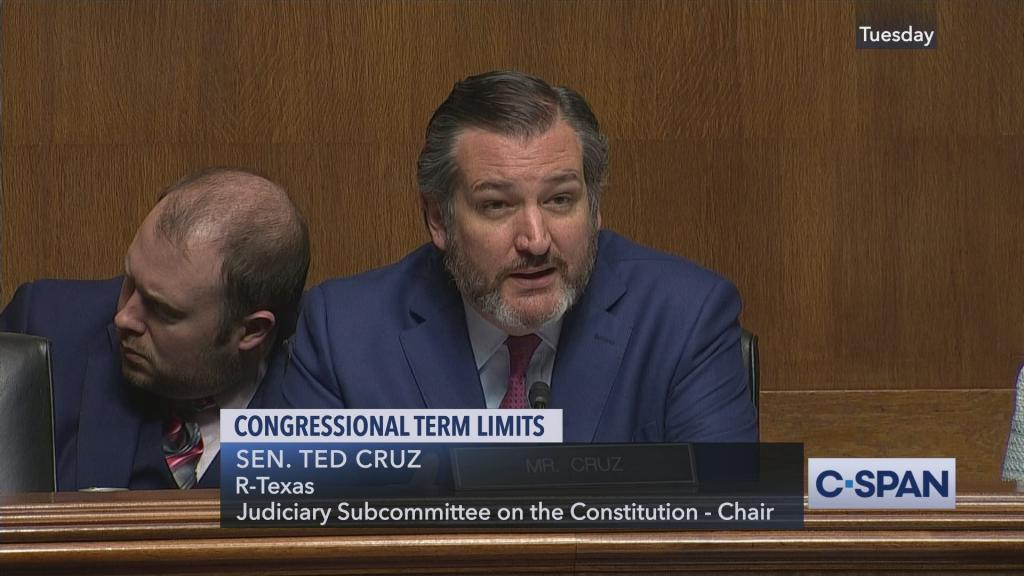
\includegraphics{../figs/CruzHearing1.jpg}}
            
            ``...members of Congress get re-elected and the system works for everyone except the American people.  This kind of self-interest builds on itself as members spend more time in office"
            
            
            \end{frame}
            
            
            \begin{frame}
            
            
            \scalebox{0.4}{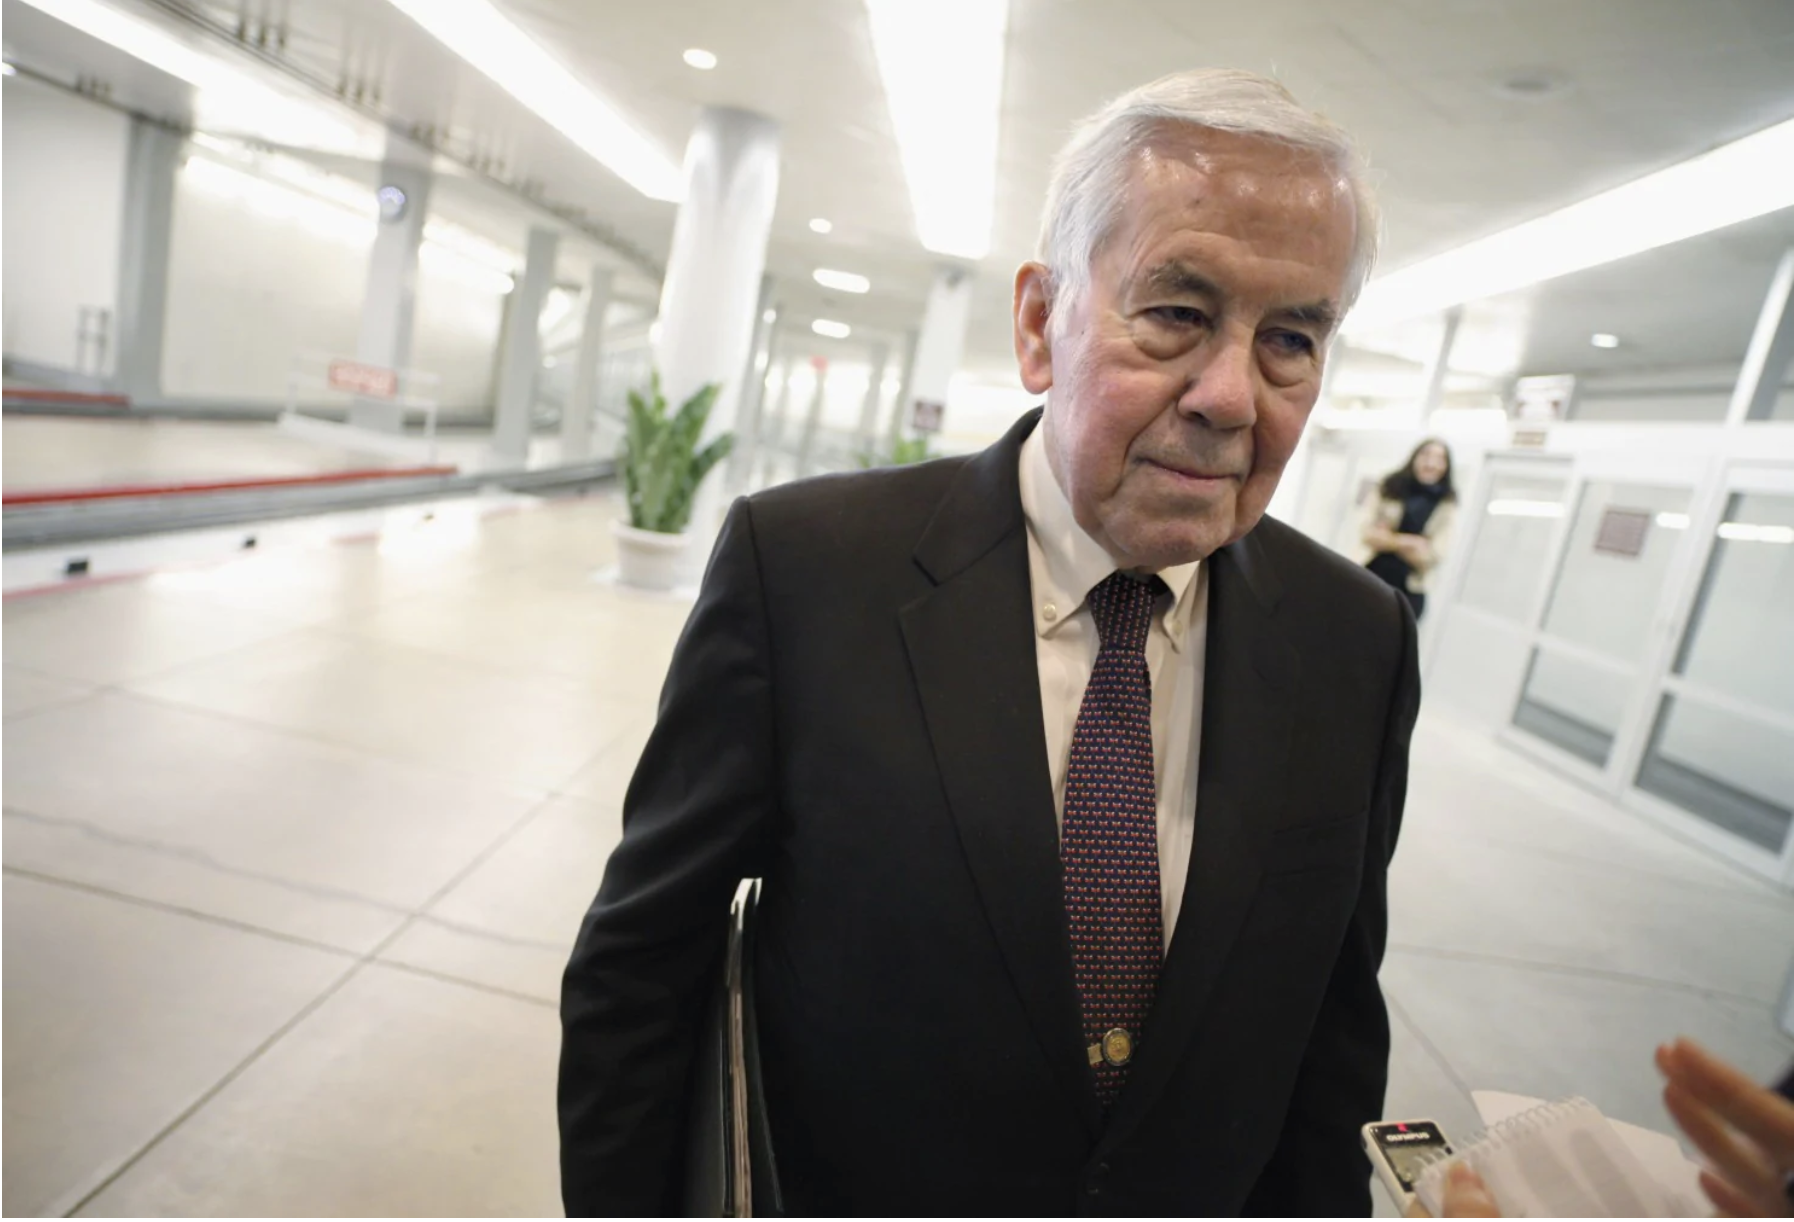
\includegraphics{../figs/DickLugar.png}}
            
            Potomac Fever (Fenno 1978) 
            
            \end{frame}
            
            
            \begin{frame}
            
            \Large 
            
            How do legislators' attention to district and constituency service change over their career?  \pause 
            
            \begin{itemize}
            \invisible<1>{\item Do constituents face a trade off between power in Washington and ``delivery of goods"?} \pause 
            \invisible<1-2>{\item Cost of new representatives: start up costs for constituency service? }  
            \end{itemize}
            
            \end{frame}
            
            
            
            \begin{frame}
            \frametitle{Delivering the Goods with Constituency Service}
            
            \begin{itemize}
            \item[-] Comprehensive census of Congressional correspondence with bureaucracy \pause 
            \begin{itemize}
            \invisible<1>{\item \input{/users/eleanorpowell/correspondence/data/foia_requests} Freedom of Information Act Requests (294 components) from 2007-2017 } \pause 
            \invisible<1-2>{\item \input{/users/eleanorpowell/correspondence/data/n} Contacts (so far)} \pause 
            \invisible<1-3>{\item Builds upon important prior work that focused on specific legislator-agency pairs (\textcolor{gray}{Ritchie 2017; Mills and Kalaf-Hughes, 2015; Lowande, 2018})} \pause 
            \end{itemize}
            \invisible<1-4>{\item[-] Legislators' contact with agencies: 90\% constituency service} \pause 
          \invisible<1-5>{\item[-] Increased power and experience$\leadsto$ increased constituency service } \pause 
          \begin{itemize}
          \invisible<1-6>{\item[-] Difference-in-differences, Legislator x Agency level} \pause 
          \invisible<1-7>{\item[-] Increased power from committee assignment$\leadsto$ increased number of contacts} \pause 
          \invisible<1-8>{\item[-] New legislators$\leadsto$ fewer contacts, Experience $\leadsto$ more contacts} \pause 
          \end{itemize}
          \invisible<1-9>{\item[-] Small (no) change in type of contact, Little evidence due to demand} \pause 
          \invisible<1-10>{\item[-] Increased power and experience$\leadsto$ greater policy influence and district benefits} 
          \end{itemize}
          
          
          
          \end{frame}
          
          
          
          \begin{frame}
          \frametitle{Legislator Attention to the District and Constituency Service}
          
          Competing expectations about how power and experience affect service:  \pause 
          \begin{itemize}
          \invisible<1>{\item Term limit advocates: legislators attention drifts away from district and towards Washington} \pause 
          \invisible<1-2>{\item Multitask + Selection models of representation (e.g. Ashworth and Bueno de Mesquita 2006): increases in legislators' budgets$\leadsto$increased constituency service  } \pause 
            \invisible<1-3>{\item Constituent demand: legislators merely respond to requests from district, little choice} \pause 
            \end{itemize}
            
            
            \end{frame}
            
            
            
            \begin{frame}
            \frametitle{A Census of Federal Contacts}
            
            \only<1-3, 9->{Constituency service: ``provid[e] help to individuals, groups, and localities in coping with the federal government" (Fenno 1978)  
            \begin{itemize}
            \invisible<1>{\item Identify department, agencies, and subagencies} 
            \invisible<1-2>{\item Freedom of Information Act: All contacts from members of Congress 2007-2017} \pause 
            \invisible<1-8>{\item Clean, merge with Congressional data} 
            \invisible<1-9>{\item Hand code $\approx$ 1/2 of contacts } 
            \begin{itemize}
            \invisible<1-10>{\item[-] Individual (constituency service)} 
            \invisible<1-10>{\item[-] Corporate (constituency service)}
            \invisible<1-10>{\item[-] 501c3/Local Government (constituency service)}
            \invisible<1-10>{\item[-] General policy }
            \invisible<1-10>{\item[-] Corporate policy } 
            \end{itemize}
            \end{itemize}
            }
            
            \only<4>{\begin{scriptsize}
            \input{../tables/FOIA_Table.tex}
            \end{scriptsize}}
            
            \only<5>{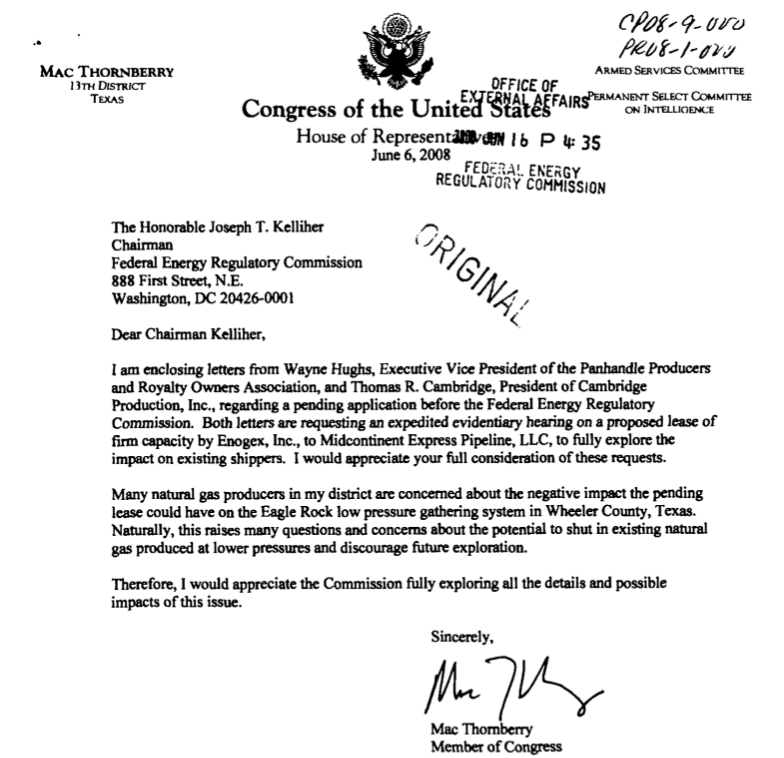
\includegraphics[width = \textwidth]{../../../correspondence/FERC.png}} 
            
            
            \only<6>{Department of Homeland Security Immigration and Customs Enforcement (ICE)
            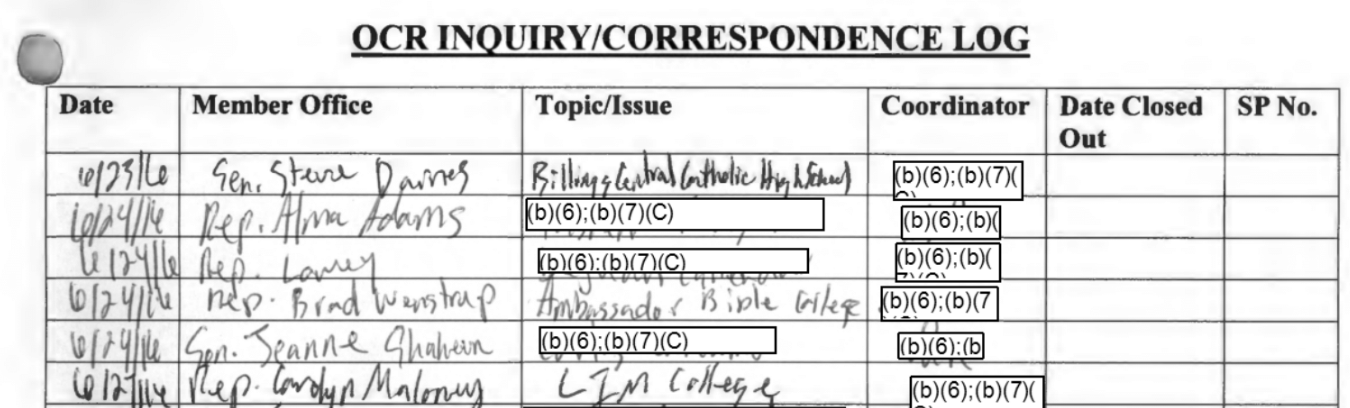
\includegraphics[width = \textwidth]{../../../correspondence/ICE.png}}
            
            
            \only<7>{Environmental Protection Agency
            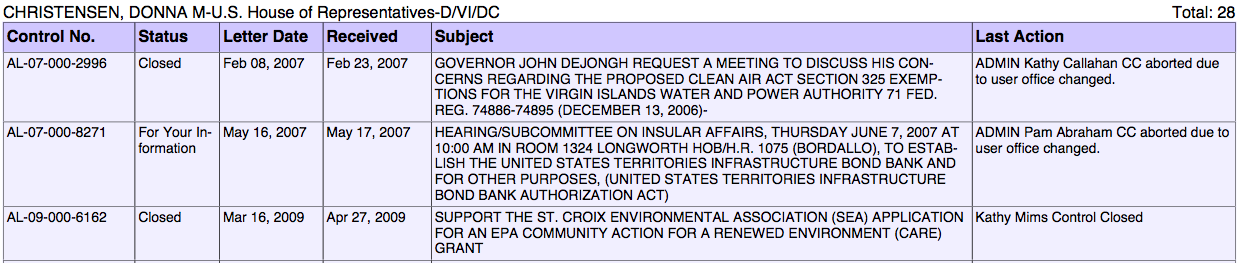
\includegraphics[width = \textwidth]{../../../correspondence/EPA.png}}
            
            \only<8>{ Department of Homeland Security Immigration and Customs Enforcement (ICE)
            
            \includegraphics[width = \textwidth]{../figs/schwartz.png} }
            
            
            \pause \pause \pause \pause \pause \pause \pause \pause \pause 
            
            
            \end{frame}
            
            
            
            
            
            
            
            
            
            %\frametitle{Correspondence Data}
            % For example, here Rep. Thornberry, chair of armed services committee is writing to Federal Energy Regulatory Commission on behalf of two companies in his district, asking for extra scrutiny on a another company's permit application. 
            
            % We have several thousand such letters written to this agency, which we use optical content recognition to extract the text. If they do not have metadata like the sender's name and date, we extract it from the text of the letter or discription of the letter.
            
            %\frametitle{Correspondence Data}
            
            
            
            
            %\frametitle{Correspondence Data}
            
            % rich and informative summaries like those kept by the EPA. Here, Rep Donna writes about a regulatory exemption for a power plant, to alert EPA to a hearing, and in support of a nonprofit grant application.
            
            \begin{frame}
            \frametitle{New Facts About Legislator Contact with Federal Agencies}
            
            \only<1>{\scalebox{0.5}{\includegraphics{../figs/TypeHistogram1.pdf}}}
            
            \only<2>{\scalebox{0.5}{\includegraphics{../figs/TypeHistogram2.pdf}}}
            
            \only<3>{\scalebox{0.3}{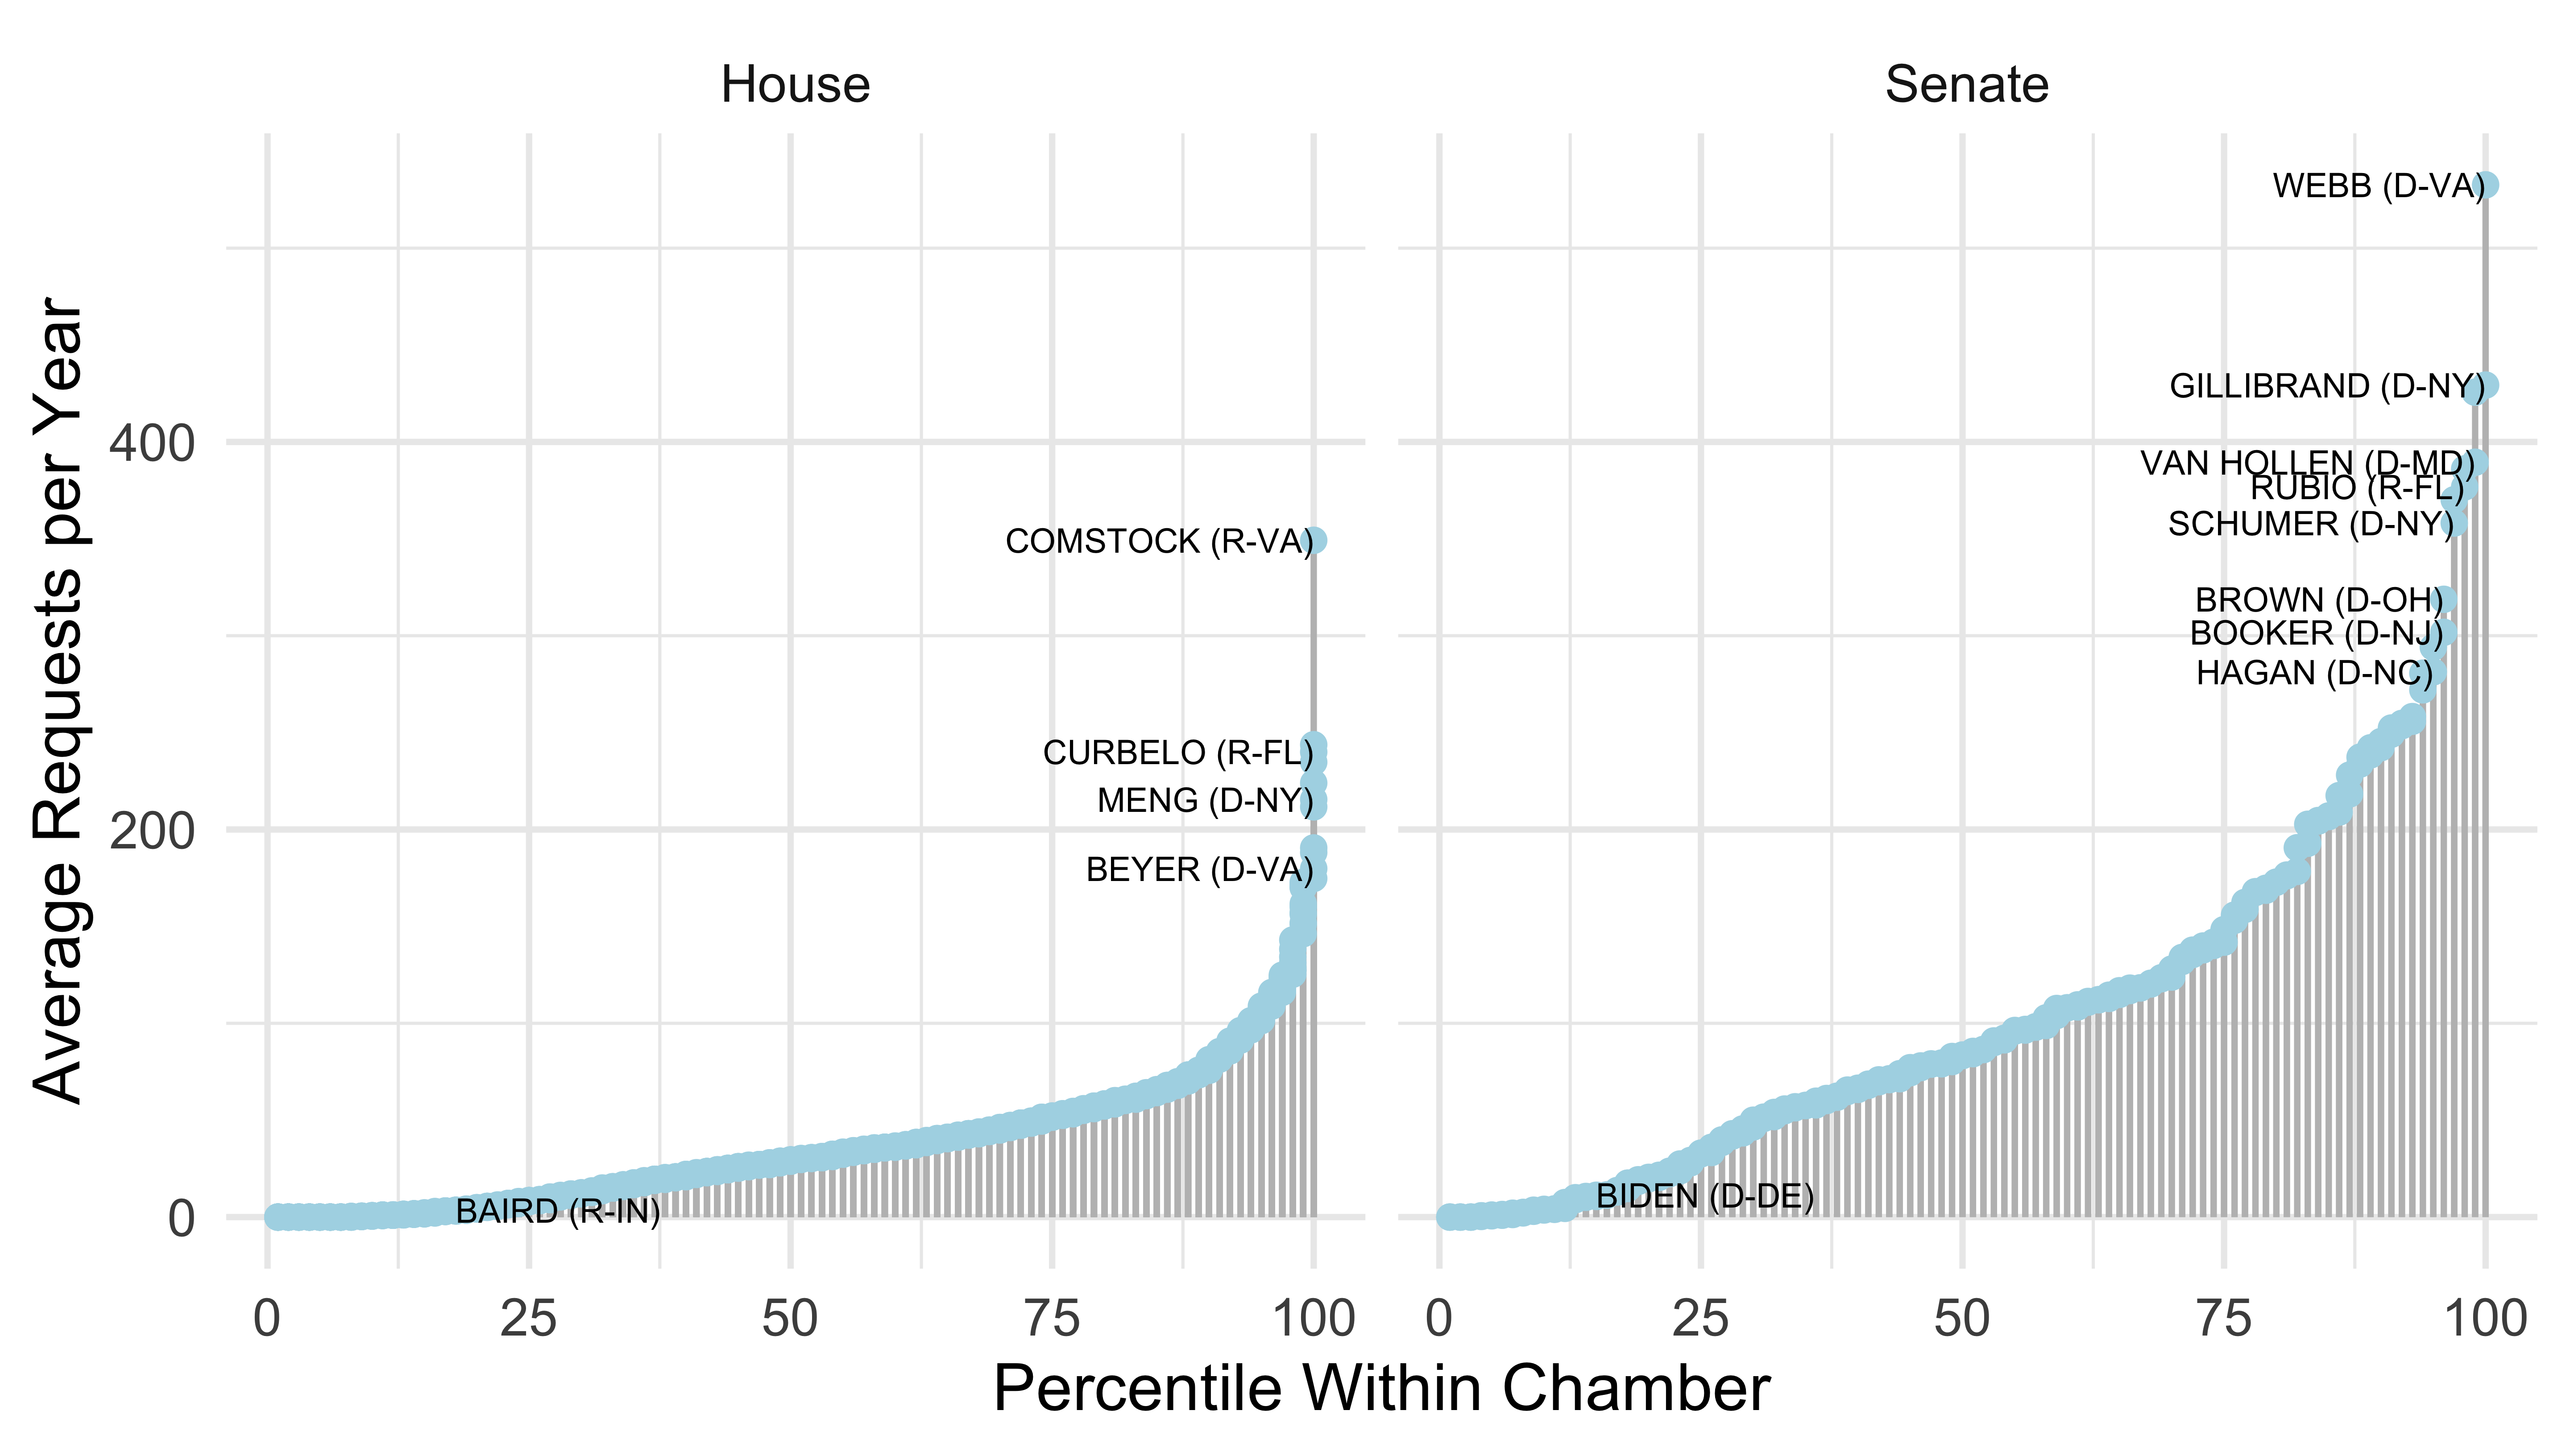
\includegraphics{/users/eleanorpowell/correspondence/Figs/percentiles-1}}}
            
            \only<4>{\scalebox{0.3}{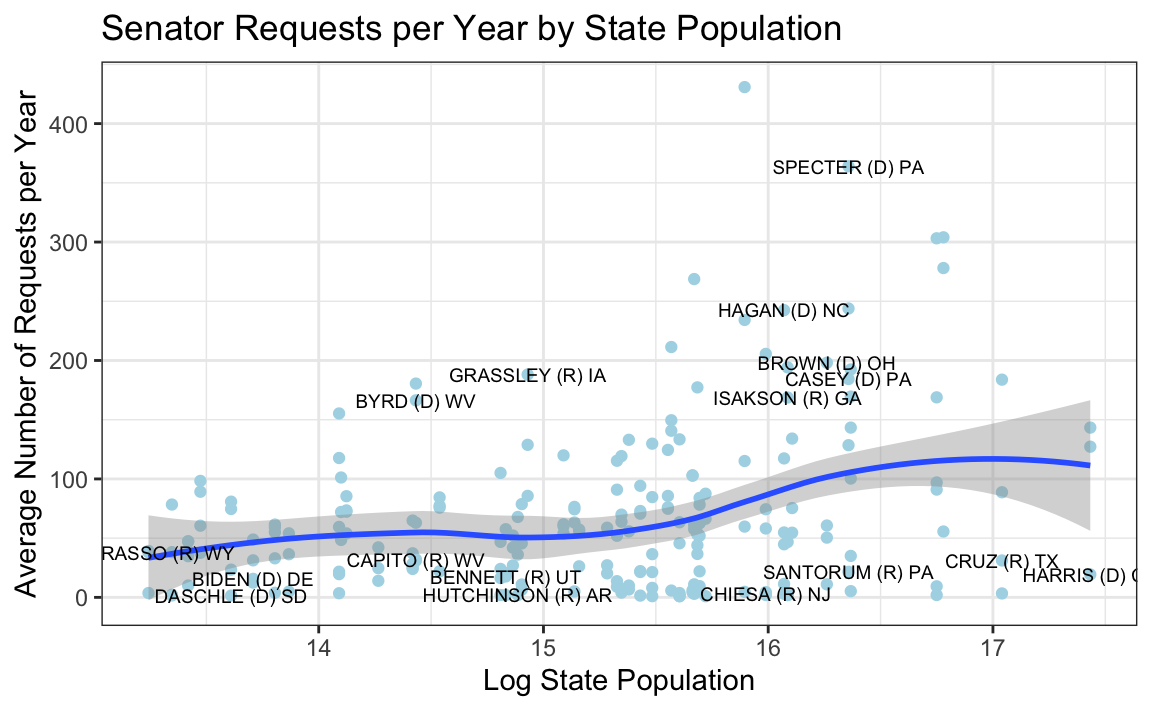
\includegraphics{/users/eleanorpowell/correspondence/Figs/population-1}}}
            
            \only<5>{
            District demographics are correlated with types of requests legislators make
            \begin{itemize}
            \item Higher proportion of veterans $\leadsto$ more requests to VA
            \item Higher proportion of residents over 65 $\leadsto$ more requests to SSA 
            \end{itemize}		
            }
            
            \end{frame}
            
            \begin{frame}
            \frametitle{Assessing the Effect of Committee Power and Experience}
            
            Goal: estimate effect of prestige and experience in Congress on constituency service \pause 
            
            \begin{itemize}
            \invisible<1>{\item Cross-sectional comparison} \pause 
            \begin{itemize}
            \invisible<1-2>{\item[-] Descriptive differences are important} \pause
            \invisible<1-2>{\item[-] Conflates ability with position } \pause
            \invisible<1-2>{\item[-] Difficult to identify a set of covariates to disentangle} \pause
            \end{itemize}
            \invisible<1-3>{\item Panel Design} \pause 
            \begin{itemize}
            \invisible<1-4>{\item[-] Difference-in-differences at the legislator-agency level} \pause 
            \invisible<1-4>{\item[-] Examine within legislator-agency change} \pause 
            \invisible<1-4>{\item[-] Include time-varying characteristics} 
            \end{itemize}		
            \end{itemize}
            
            \end{frame}
            
            
            
            \begin{frame}
            \frametitle{Estimating Effect of Increasing Committee Prestige on Contacts}
            
            \begin{eqnarray}
            Y_{ijt} & = & \beta \text{Committee Position}_{it}   + \gamma_{ij} +  \delta_{t} + \sum_{s = 1}^{S} \eta_{s} \text{tenure}_{s[it]} + m_{it} + p_{it} +  \epsilon_{ijt}  \nonumber 
            \end{eqnarray}
            
            Where: \pause 
            \begin{itemize}
            \invisible<1>{\item  $Y_{ijt} = $ Number of contacts between legislator $i$ and agency $j$ in year $t$} \pause 
            \invisible<1-2>{\item $\beta = $ Estimated causal effect of obtaining committee position } 
            \begin{itemize}
            \invisible<1-2>{	\item[1)] Chair of committee}
            \invisible<1-2>{	\item[2)] Ranking member }
            \invisible<1-2>{	\item[3)] Prestige committee assignment}
            \invisible<1-2>{	\item[4)] Oversight committee assignment}\pause 
            \end{itemize}
            \invisible<1-3>{\item  $\gamma_{ij} = $ Legislator $i$ x Agency $j$ fixed effect }
            \invisible<1-3>{\item  $\delta_{t} = $ Year $t$ fixed effect}\pause
            \invisible<1-4>{\item $m_{it}, p_{it},\sum_{s = 1}^{S} \eta_{s} \text{tenure}_{s[it]} $ time varying controls } \pause 
            \end{itemize}
            
            \invisible<1-5>{Standard errors clustered at legislator-agency level} %(same results if clustered at legislator level)}
            
            
            \end{frame}
            
            
            \begin{frame}
            
            \begin{footnotesize}
            \begin{tabular}{l*{4}{c}}
\toprule
                    &\multicolumn{1}{c}{(1)}&\multicolumn{1}{c}{(2)}&\multicolumn{1}{c}{(3)}&\multicolumn{1}{c}{(4)}\\
\midrule
Committee Chair     &       0.522&       0.243&       0.243&      0.0377\\
                    &    (0.0826)&    (0.0747)&    (0.0747)&   (0.00658)\\
Ranking Member      &       0.652&       0.137&       0.137&      0.0289\\
                    &    (0.0887)&    (0.0683)&    (0.0683)&   (0.00641)\\
Prestige Committee  &       0.425&      0.0798&      0.0798&      0.0188\\
                    &    (0.0324)&    (0.0269)&    (0.0269)&   (0.00467)\\
Oversight Committee &       0.420&       0.161&       0.160&      0.0565\\
                    &    (0.0296)&    (0.0190)&    (0.0192)&   (0.00324)\\
\midrule
Tenure              &  \checkmark&  \checkmark&  \checkmark&  \checkmark\\
Majority, President's Party&  \checkmark&  \checkmark&  \checkmark&  \checkmark\\
Legislator $\times$ Agency Fixed Effects&            &  \checkmark&  \checkmark&  \checkmark\\
Year Fixed Effects  &            &  \checkmark&  \checkmark&  \checkmark\\
All Legislators     &  \checkmark&  \checkmark&            &            \\
Serve At Least Second Term&            &            &  \checkmark&            \\
Dependent Variable  &       Count&       Count&       Count&Log(Count + 1)\\
Observations        &      337610&      337610&      330215&      337610\\
\bottomrule
\multicolumn{5}{l}{\footnotesize Robust standard errors in parentheses, clustered at legislator x agency level}\\
\end{tabular}

            \end{footnotesize}
            
            \end{frame}
            
            \begin{frame}
            \frametitle{Within-Legislator Comparison of Tenure Effects}
            
            
            \begin{eqnarray}
            Y_{ijt} & = & \sum_{s=1}^{6} \beta_{s} \text{tenure}_{s[it]} + \gamma_{ij} +  \delta_{t}  + m_{it} + p_{it} +  \epsilon_{ijt} \nonumber 
            \end{eqnarray} 
            
            
            
            Where: \pause 
            \begin{itemize}
            \invisible<1>{\item  $Y_{ijt} = $ Number of contacts between legislator $i$ and agency $j$ in year $t$} \pause 
            \invisible<1-2>{\item $\beta_{s} = $ Estimated causal effect of tenure year $s$ } \pause 
            \invisible<1-3>{\item  $\gamma_{ij} = $ Legislator $i$ x Agency $j$ fixed effect }
            \invisible<1-3>{\item  $\delta_{t} = $ Year $t$ fixed effect} \pause 
            \invisible<1-4>{\item $m_{it}, p_{it}$ time varying controls for majority and same party as president }\pause 
            \end{itemize}
            
            \invisible<1-5>{Standard errors clustered at legislator-agency level } 
            
            \end{frame}
            
            
            \begin{frame}
            
            \begin{footnotesize}
            \begin{tabular}{l*{4}{c}}
\toprule
                    &\multicolumn{1}{c}{(1)}&\multicolumn{1}{c}{(2)}&\multicolumn{1}{c}{(3)}&\multicolumn{1}{c}{(4)}\\
\midrule
First Year          &      -0.478&      -0.179&      -0.183&     -0.0317\\
                    &    (0.0349)&    (0.0347)&    (0.0351)&   (0.00527)\\
Second Year         &      -0.344&     -0.0665&     -0.0630&   -0.000440\\
                    &    (0.0375)&    (0.0335)&    (0.0337)&   (0.00510)\\
Third Year          &      -0.274&    -0.00694&    -0.00697&     0.00662\\
                    &    (0.0376)&    (0.0328)&    (0.0328)&   (0.00482)\\
Fourth Year         &      -0.237&      0.0200&      0.0200&      0.0126\\
                    &    (0.0409)&    (0.0310)&    (0.0310)&   (0.00470)\\
Fifth Year          &      -0.238&    0.000539&    0.000506&   -0.000442\\
                    &    (0.0388)&    (0.0296)&    (0.0296)&   (0.00434)\\
Sixth Year          &      -0.220&      0.0204&      0.0204&     0.00242\\
                    &    (0.0401)&    (0.0278)&    (0.0278)&   (0.00414)\\
\midrule
Majority, President's Party&  \checkmark&  \checkmark&  \checkmark&  \checkmark\\
Legislator $\times$ Agency Fixed Effects&            &  \checkmark&  \checkmark&  \checkmark\\
Year Fixed Effects  &            &  \checkmark&  \checkmark&  \checkmark\\
All Legislators     &  \checkmark&  \checkmark&            &  \checkmark\\
Serve At Least Second Term&            &            &  \checkmark&            \\
Dependent Variable  &       Count&       Count&       Count&Log(Count + 1)\\
Observations        &      337610&      337610&      330215&      337610\\
\bottomrule
\multicolumn{5}{l}{\footnotesize Robust standard errors in parentheses, clustered at legislator x agency level}\\
\end{tabular}

            \end{footnotesize} 
            
            \end{frame}
            
            
            \begin{frame}
            \frametitle{Within-District Comparison of Tenure Effects}
            
            \begin{eqnarray}
            Y_{it} & = & \beta_{1}\text{New Member}_{it} + \sum_{s = 2}^{6} \beta_{s} \text{tenure}_{s[it]} + \overbrace{\gamma_{i}}^{\text{District}} + \underbrace{\delta_{t}}_{\text{Year}} + \epsilon_{it} \nonumber 
            \end{eqnarray}
            
            Where: \pause 
            \begin{itemize}
            \invisible<1>{\item $Y_{it} = $ Number of contacts in district $i$ and year $t$ } \pause 
            \invisible<1-2>{\item $\beta_{1} = $ effect of a new member } \pause 
            \invisible<1-3>{\item $\beta_{s} = $ effect of member in year 2-6} 
            \end{itemize}	
            
            
            
            \end{frame}
            
            
            \begin{frame}
            
            \begin{footnotesize}
            \begin{center}
            \begin{tabular}{l*{4}{c}}
\toprule
                    &\multicolumn{1}{c}{(1)}&\multicolumn{1}{c}{(2)}&\multicolumn{1}{c}{(3)}&\multicolumn{1}{c}{(4)}\\
\midrule
New Legislator      &      -35.23&      -35.55&      -14.89&      -123.5\\
                    &     (4.445)&     (4.500)&     (2.627)&     (13.84)\\
Legislator 2nd Year &      -23.75&      -20.31&      -4.402&      -79.99\\
                    &     (4.464)&     (3.949)&     (2.662)&     (11.34)\\
Legislator 3rd Year &      -13.08&      -13.53&      -1.630&      -49.48\\
                    &     (4.886)&     (4.448)&     (2.586)&     (16.07)\\
Legislator 4th Year &      -12.43&      -9.077&       0.268&      -26.92\\
                    &     (5.216)&     (4.276)&     (2.736)&     (16.30)\\
Legislator 5th Year &      -14.92&      -11.58&      -3.810&      -31.58\\
                    &     (4.416)&     (3.591)&     (2.128)&     (13.11)\\
Legislator 6th Year &      -13.56&      -5.216&      -1.638&      -2.500\\
                    &     (5.104)&     (3.790)&     (2.239)&     (14.46)\\
\midrule
District Fixed Effects&            &  \checkmark&  \checkmark&  \checkmark\\
Year Fixed Effects  &            &  \checkmark&  \checkmark&  \checkmark\\
All Districts       &  \checkmark&  \checkmark&            &            \\
House Only          &            &            &  \checkmark&            \\
Senate Only         &            &            &            &  \checkmark\\
Observations        &        6578&        6578&        5338&        1240\\
\bottomrule
\multicolumn{5}{l}{\footnotesize Robust standard errors in parentheses, clustered at district level}\\
\end{tabular}

            \end{center}
            \end{footnotesize}
            
            \end{frame}
            
            \begin{frame}
            \frametitle{Increased Service or Increased Contacts?}
            
            Do legislators change what types of requests?  \pause 
            \begin{itemize}
            \invisible<1>{\item[-] Concern: new requests are about policy, not service} \pause 
            \invisible<1-2>{\item[-] Cannot identify causal effect on type} \pause
            \invisible<1-3>{\item[-] Descriptive quantity: show proportion of requests still constituent service remains high} \pause 
            \end{itemize}	
            \invisible<1-4>{Empirical strategy: } \pause 
            \begin{itemize}
            \invisible<1-5>{\item Dependent variable: $\frac{\text{No. Constituent Service Contacts}}{\text{No.Constituent Service Contacts + No. Policy }  }$}\pause 
            \invisible<1-6>{\item Assess differences on committee assignment, tenure} 
            \end{itemize}	
            
            
            
            \end{frame}
            
            
            
            
            
            \begin{frame}
            \frametitle{Dependent Variable: Proportion of Contacts Constituency Service}
            
            \only<1>{
            \begin{scriptsize}
            \begin{tabular}{l*{2}{c}}
\toprule
                    &\multicolumn{1}{c}{(1)}&\multicolumn{1}{c}{(2)}\\
\midrule
First Year          &      0.0286&      0.0714\\
                    &   (0.00888)&    (0.0128)\\
Second Year         &      0.0326&      0.0591\\
                    &   (0.00785)&    (0.0123)\\
Third Year          &      0.0315&      0.0567\\
                    &   (0.00775)&    (0.0116)\\
Fourth Year         &      0.0124&      0.0354\\
                    &   (0.00876)&    (0.0121)\\
Fifth Year          &      0.0101&      0.0270\\
                    &    (0.0100)&    (0.0135)\\
Sixth Year          &      0.0233&      0.0303\\
                    &   (0.00920)&    (0.0103)\\
Intercept           &       0.857&       0.829\\
                    &   (0.00418)&   (0.00655)\\
\midrule
Majority            &            &  \checkmark\\
Legislator Fixed Effects&            &  \checkmark\\
Year Fixed Effects  &            &  \checkmark\\
Observations        &        5902&        5876\\
\bottomrule
\multicolumn{3}{l}{\footnotesize Robust standard errors in parentheses, clustered at legislator level}\\
\end{tabular}

            \end{scriptsize}
            }
            
            \only<2>{
            \begin{scriptsize}
            \begin{tabular}{l*{2}{c}}
\toprule
                    &\multicolumn{1}{c}{(1)}&\multicolumn{1}{c}{(2)}\\
\midrule
Prestige            &      0.0313&     0.00445\\
                    &   (0.00614)&    (0.0110)\\
Chair               &     -0.0498&     -0.0662\\
                    &    (0.0105)&    (0.0144)\\
Ranking Minority    &     -0.0231&     -0.0268\\
                    &   (0.00942)&    (0.0135)\\
Oversight Committee &     0.00385&     0.00160\\
                    &   (0.00979)&    (0.0110)\\
Intercept           &       0.852&       0.848\\
                    &    (0.0102)&    (0.0125)\\
\midrule
Majority            &            &  \checkmark\\
Legislator Fixed Effects&            &  \checkmark\\
Year Fixed Effects  &            &  \checkmark\\
Observations        &        5876&        5876\\
\bottomrule
\multicolumn{3}{l}{\footnotesize Robust standard errors in parentheses, clustered at legislator level}\\
\end{tabular}

            \end{scriptsize}
            }
            
            
            \end{frame}
            
            \begin{frame}
            \frametitle{Summary of Results}
            
            
            \Large 
            \begin{itemize}
            \item Increased power in Congress $\leadsto$ More contacts
            \item More experience in Congress $\leadsto$ More contacts
            \item Increased contacts $\leadsto$ more constituency service
            \end{itemize}
            
            \end{frame}
            
            
            
            
            \begin{frame}
            \frametitle{Constituent Demand}
            
            Are legislators merely reacting to constituent demand? \pause 
            \begin{itemize}
            \invisible<1>{\item Research design addresses static and slow-moving demand} \pause 
            \invisible<1-2>{\item Demand for constituency service can (and often is) created$\leadsto$ different mechanism} \pause 
            \invisible<1-3>{\item Possible constituents' requests track changes in power and experience} \pause 
          \end{itemize}
          
          \invisible<1-4>{Test two implications of constituent demand explaining results } \pause 
          \begin{itemize}
          \invisible<1-5>{\item[1)] Do other legislators contact more when they have new legislator in same state? } \pause 
          \invisible<1-6>{\item[2)] Does name recognition increase with prestige and power?} 
          \end{itemize} 
          
          
          \end{frame}
          
          
          \begin{frame}
          \frametitle{Who Do Constituents Ask for Help}
          
          
          Where do constituents redirect constituency service requests?  
            
            \begin{itemize}
          \item New legislators make fewer contacts with federal agencies
          \item Demand interpretation: fewer request from constituents
          \item If constituents still need help: may direct requests to incumbent legislators
          \item Legislators with new colleagues should see \alert{increase} in contacts 
          \end{itemize}
          
          Assess how new members in state affect representative and senator contacting behavior
          
          
          \end{frame}
          
          
          \begin{frame}
          \frametitle{Little Evidence of Spillover}
          \begin{tabular}{l*{4}{c}}
\toprule
                    &\multicolumn{1}{c}{(1)}&\multicolumn{1}{c}{(2)}&\multicolumn{1}{c}{(3)}&\multicolumn{1}{c}{(4)}\\
\midrule
Proportion New Legislators&       5.143&            &      -1.494&            \\
                    &     (8.089)&            &     (20.06)&            \\
At Least One New Legislator&            &       1.625&            &       3.847\\
                    &            &     (2.031)&            &     (4.812)\\
\midrule
District Fixed Effects&  \checkmark&  \checkmark&  \checkmark&  \checkmark\\
Year Fixed Effects  &  \checkmark&  \checkmark&  \checkmark&  \checkmark\\
Senators Only       &            &            &  \checkmark&  \checkmark\\
Observations        &        6080&        6080&        1182&        1182\\
\bottomrule
\multicolumn{5}{l}{\footnotesize Robust standard errors in parentheses, clustered at district level}\\
\end{tabular}

          
          
          \end{frame}
          
          
          \begin{frame}
          \frametitle{Assessing Name Recognition}
          
          Constituents could direct attention at better known legislators
          
          \begin{itemize}
          \item[1)] Does name recognition increase with prestige and tenure? 
            \item[2)] \alert{Do better recognized legislators receive more constituency service requests ?}
          \end{itemize}
          
          Measuring name recognition: 
            \begin{itemize}
          \item CCES cumulative file (2006-2018)
          \item Use approval question: ``Never Heard/Not Sure" (Don't Recognize), Otherwise (Recognize)
          \end{itemize}
          
          \end{frame}
          
          
          \begin{frame}
          \frametitle<1>{Weak Relationship Between Name Recognition and Constituent Service Requests: House}
          \frametitle<2>{Weak Relationship Between Name Recognition and Constituent Service Requests: Senate}
          
          
          \only<1>{\scalebox{0.5}{\includegraphics{../Figs/HouseRecFig.pdf}}}
          \only<2>{\scalebox{0.5}{\includegraphics{../Figs/SenateRecFig.pdf}}}
          
          %\only<1>{\begin{scriptsize}
          %\begin{tabular}{l*{2}{c}}
\toprule
                    &\multicolumn{1}{c}{(1)}&\multicolumn{1}{c}{(2)}\\
\midrule
Second Year         &     -0.0385&     -0.0230\\
                    &   (0.00642)&   (0.00641)\\
Fourth Year         &     -0.0263&    0.000275\\
                    &   (0.00646)&   (0.00682)\\
Sixth Year          &     -0.0281&     -0.0112\\
                    &   (0.00676)&   (0.00634)\\
Eighth Year         &     -0.0132&     0.00132\\
                    &   (0.00663)&   (0.00674)\\
\midrule
Legislator Fixed Effects&            &  \checkmark\\
Year Fixed Effects  &            &  \checkmark\\
Observations        &        3667&        3667\\
\bottomrule
\multicolumn{3}{l}{\footnotesize Robust standard errors in parentheses, clustered at legislator level}\\
\end{tabular}

          %\end{scriptsize}}
          
          %\only<2>{\begin{scriptsize}
          %\begin{tabular}{l*{2}{c}}
\toprule
                    &\multicolumn{1}{c}{(1)}&\multicolumn{1}{c}{(2)}\\
\midrule
Prestige            &      0.0249&   -0.000101\\
                    &   (0.00506)&   (0.00669)\\
Chair               &      0.0342&    -0.00775\\
                    &   (0.00770)&   (0.00627)\\
Ranking Minority    &      0.0299&    -0.00381\\
                    &   (0.00866)&   (0.00699)\\
Oversight Committee &     0.00503&     -0.0144\\
                    &   (0.00591)&   (0.00537)\\
Majority Party      &    0.000224&    -0.00153\\
                    &   (0.00381)&   (0.00303)\\
President's Party   &      0.0254&      0.0221\\
                    &   (0.00312)&   (0.00312)\\
\midrule
Legislator Fixed Effects&            &  \checkmark\\
Year Fixed Effects  &            &  \checkmark\\
Observations        &        3667&        3667\\
\bottomrule
\multicolumn{3}{l}{\footnotesize Robust standard errors in parentheses, clustered at legislator level}\\
\end{tabular}

          %\end{scriptsize}}
          
          \end{frame}
          
          \begin{frame}
          \frametitle{Conclusion}
          
          More Experience, More Power $\leadsto$ More constituency service
          
          \begin{itemize}
          \item No tradeoff: As legislators acquire power, also ``deliver the goods" to district
          \item \alert{Costs} of electing new legislators 
          \item Little evidence for Potomac Fever
          \end{itemize}
          
          Broad set of projects 
          \begin{itemize}
          \item Lettermarking and earmark bans
          \item Company donations and constituent service requests
          \item Ideological nature of federal contacts
          \item Content analysis of what legislators ask for
          \end{itemize}	
          
          
          
          \end{frame}
          
          
          
          
          \end{document}